
% ==================================================
%	Theorie
% ==================================================

\section{Theorie}

Die Tomographie ist ein bildgebendes Verfahren, also eine Technik, die
Verteilung physikalischer Eigenschaften, wie z.B.~den Absorptionskoeffizienten,
eines Objektes zu visualisieren. Durch verschiedene Querschnittsbilder kann so
die Struktur des Objektes ermittelt werden. In diesem Versuch wird zur
Untersuchung der Struktur der Würfel $\gamma$-Strahlung eines
$^{60}\text{Co}$-Strahlers verwandt.
Der Würfel wird nun aus einer Richtung bestrahlt, wobei die Strahlung damit in
seiner Intensität geschwächt wird.
Wie stark die Intensität geschwächt wird, hängt von
den in dem Würfel vorkommenden Materialien ab. Dieser Vorgang wird von
verschiedenen Richtungen wiederholt.
So kann theoretisch ein dreidimensionales Abbild des
Würfels erstellt werden kann. Die in diesem Versuch verwandten Würfel bestehen
aus $3\times 3 \times 3$ Elementarwürfel, wobei nur die mittlere Ebene
ausgemessen wird. Die Tomographie baut also auf das Verständnis der
Wechselwirkung von $\gamma$-Strahlung mit Materie auf.
Diese sollen nun kurz beschrieben werden.

% ==================================================
% 	Erzeugung von Gamma-Strahlung
% ==================================================
\subsection{Erzeugung von $\gamma$-Strahlung}
\label{sub:erzeugung_von_gamma_strahlung}

Wie eingangs erwähnt wird in diesem Versuch zur Erzeugung von
$\gamma$-Strahlung das radioaktive Isotop \Co~verwandt.
Das Zerfallsschema von \Co~ist in Abbildung~\ref{fig:Co}
dargestellt.
Hieran ist zu erkennen, dass \Co~mit einer Halbwertszeit von 5.2711 Jahren
zu fast \SI{100}{\percent} durch einen
$\beta^-$-Zerfall in einen angeregten Zustand von \Ni~zerfällt.
Dieser angeregte Zustand zerfällt schließlich unter Aussendung von
$\gamma$-Strahlung in den Grundzustand.
Hierbei ergeben sich 2 $\gamma$-Linien mit den Energien \SI{1173}{\keV} und
\SI{1322}{\keV}. Diese Linien werden zur Bestimmung der Struktur der Würfel
verwandt.
\begin{figure}[t]
  \centering
  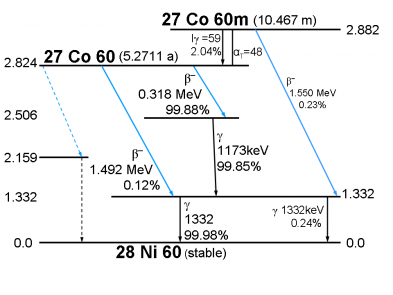
\includegraphics[scale=0.6]{bilder/393px-Co60DS.png}
  \caption{Darstellung des Zerfallsschema von $^{60}\text{Co}$.\cite{Co60}}
\label{fig:Co}
\end{figure}

\newpage
% ==================================================
% 	Wechselwirkung Gamma Strahlung
% ==================================================
\subsection{Wechselwirkung von $\gamma$-Strahlung mit Materie}
\label{sub:wechselwirkung_von_gamma_strahlung_mit_materie}

Die wesentlichen Effekte, welche bei der Wechselwirkung von $\gamma$-Strahlung
mit Materie auftrete sind
\begin{enumerate}
  \item Photo-Effekt
  \item Compton-Streuung
  \item Paar-Produktion~.
\end{enumerate}
Bei dem Photo-Effekt wird ein Photon von einem Elektron einer Atomhülle
absorbiert, wobei anschließend das Elektron aus der Atomhülle gelöst wird.
Der Compton-Effekt beschreibt hingegen die Streuung eines Photons mit einem
freien Elektron. In der Materie sind die Elektronen zwar gebunden, aber bei
einer hohen Photonenenergie im Vergleich zur Bindungsenergie kann die
Bindungsenergie vernachlässigt werden. So kann die Bindungsenergie in der
Größenordnung der Grundzustandsenergie des Wasserstoffatoms mit \SI{13.6}{\eV}
abgeschätzt werden. Somit ist dies im Vergleich mit den $\gamma$-Linien mit
$\sim \SI{1100}{\keV}$ vernachlässigbar und die Elektronen können als frei
betrachtet werden.
Die Paar-Produktion ist dagegen ein Prozess in dem ein Photon in ein Elektron
und ein Positron übergeht. Aufgrund der Impulserhaltung kann dies nur durch
Anwesenheit eines dritten Körpers geschehen. Zudem muss die Energie des Photons
mindestens zwei mal die Ruheenergie des Elektrons bzw.~des Positrons betragen.
Mit der Ruheenergie von $\sim \SI{0.5}{MeV}$ muss das Photon ca. \SI{1}{\MeV}
betragen. Die $\gamma$-Linien von \Co~liegen aber gerade knapp darüber.
Zudem nimmt die Wahrscheinlichkeit der Paarbildung mit der Photonenenergie zu,
sodass die Paar-Produktion eine untergeordnete Rolle spielt.
Somit sind die wesentliche Effekte in diesem Versuch der Photo-Effekt und
der Compton-Effekt.
